\section{Particle behavior}

\subsection{Redefine stagnation}

\begin{lemma}
\label{lem:unconverge_neq_gb}
A particle won't stop moving when its personal best and global best are not the same, 
which means that 
$ \lim_{k \rightarrow \infty} v(k) \neq 0 $, if $ x^{P} \neq x^{G} $.
\begin{proof} 
There are two existing forces driving the movement of a particle, which are $ \Delta f^{G} $ and $ \Delta f^{P} $.
Thus we have
\begin{equation}
\begin{array}{lcl}
v(k+1) & = \chi ( v(k) + \Delta f^{G} (k) + \Delta f^{P} (k) ) \\
\Delta f^{G} (k) & = \phi^{G} u^{G} (k) (x^{G} - x(k)) \\
\Delta f^{P} (k) & = \phi^{P} u^{P} (k) (x^{P} - x(k)) 
\end{array}
\end{equation}
We can see that when $ \Delta f^{G} + \Delta f^{P} \neq 0 $, $ v(k)  \not \rightarrow 0 $.
When $ x^{P} \neq x^{G} $, $ \forall u^{P}(k), u^{G}(k) \in [0, 1] $, $ \not \exists x(k) $, $ \phi^{G} u^{G} (k) (x^{G} - x(k)) + \phi^{P} u^{G} (k) (x^{P} - x(k)) = 0 $.
It means that there exists no equilibrium due to the random factors $ u^{G} (k) $ and $ u^{P} (k) $. 
\end{proof}
\end{lemma}

The stagnation phenomenon is usually modeled as that the global best and personal best are not updated.
By Lemma \ref{lem:unconverge_neq_gb}, we know that in this case, the particle will never really converge.
However, in most of the cases, the personal best is highly likely to be updated if it is not the same with the global best.

Thus, we define ``stagnation'' as the global best is not updated.
In the topology in Figure \ref{fig:topology3}, the role of the global best is like a leader in the swarm, while all the particles run locally by updating the current positions and the personal best.
We can have Property \ref{prop:stagnation_decompose}.

\begin{property}
\label{prop:stagnation_decompose}
The dynamics of a swarm can be decomposed into a sequence of stagnations.
In each stagnation, the global best is not changed.
When a new global best is found, the swarm moves into a new stagnation.
\end{property}

By the topology in Figure \ref{fig:topology3}, we also notice that interactions between the particles are maintained by the update of the global best.
When the global best is not changed, the behaviors of the particles are actually decoupled.
Thus we can have Property \ref{prop:decoupled_particles}.

\begin{property}
\label{prop:decoupled_particles}
In stagnation, any two particles in a swarm has no interaction between each other.
\end{property}

By Property \ref{prop:stagnation_decompose} and Property \ref{prop:decoupled_particles}, we are able to analyze the behavior a particle in a single stagnation.
There are two types of situations in the fitness space:
\begin{itemize}
\item global best and personal best are in same hill;
\item global best and personal best are not in same hill.
\end{itemize}

\subsection{Local optimal - One hill case}

While global best and personal best are in the same hill, the search problem becomes finding the local optimal.
Due to the rule of updating the personal best and the global best, we can have Property \ref{prop:result_of_update}.

\begin{property}
\label{prop:result_of_update}
$ f(x^{G}(k)) \geq f(x^{P}(k)) \geq f(x(k)) $
\end{property}

We have $ x^{G} \neq x^{P} \implies f(x^{G}) > f(x^{P}) $ and $ x^{G} = x^{P} \implies f(x^{G}) = f(x^{P}) $.

\begin{figure}
\centering
\subfigure[Before updating personal best.] { \label{fig:one_hill_case:a}
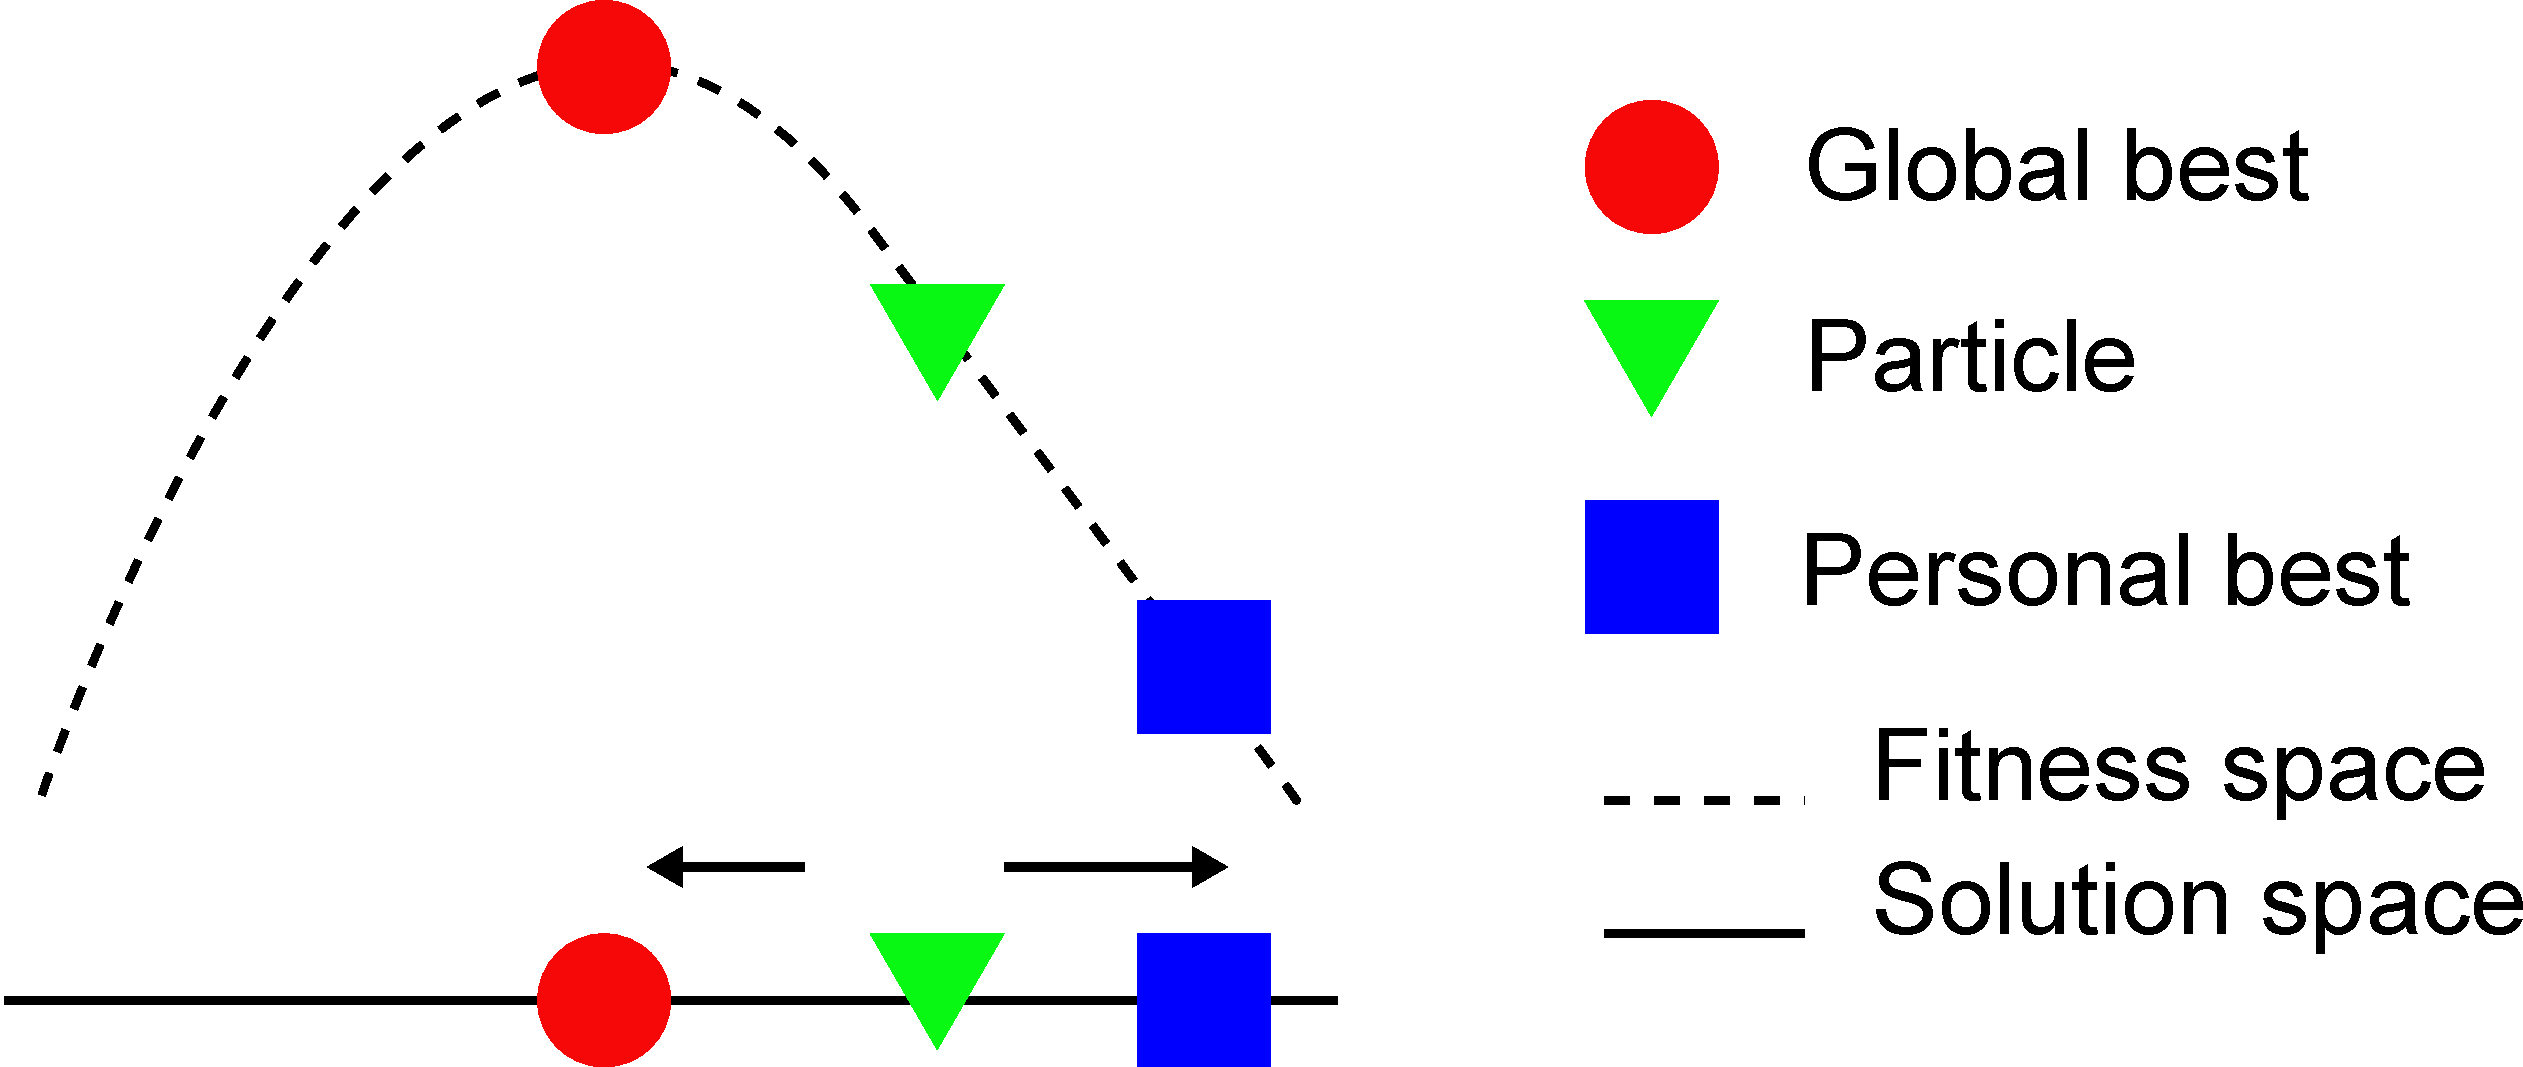
\includegraphics[width=0.47\textwidth]{one_hill_case}
}
\subfigure[After updating personal best.] { \label{fig:one_hill_case:b}
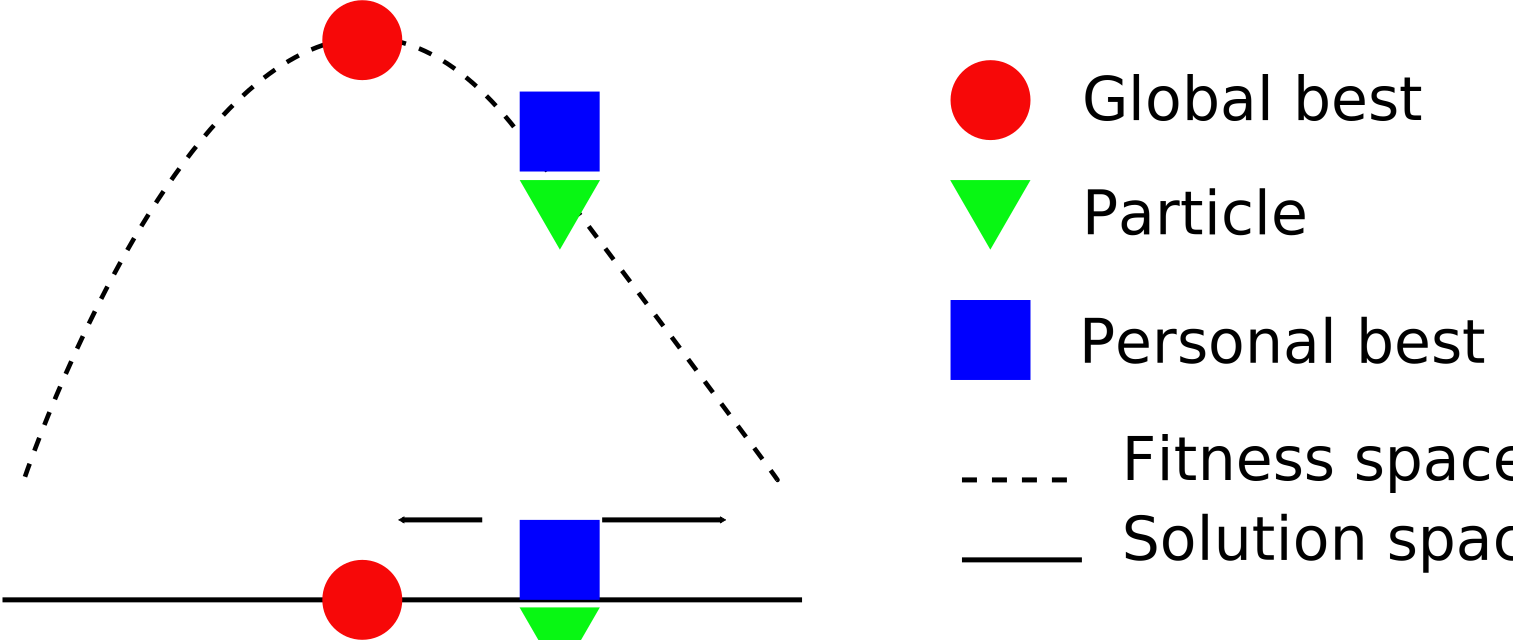
\includegraphics[width=0.47\textwidth]{one_hill_case2}
}
\caption{One hill case.}
\label{fig:one_hill_case}
\end{figure}

\begin{lemma}
\label{lem:one_hill:xp_to_xg}
Let $ x^{G} $ be fixed. 
When $ x^{P}(k) \neq x^{G} $, $ x^{P}(k) \rightarrow x^{G} $ as $ k \rightarrow \infty $.
\begin{proof}
Define the distance 
\end{proof}
\end{lemma}

\begin{lemma}
When $  x^{G} = x^{P} $, $ x(k) \rightarrow x^{G} $ as $ k \rightarrow \infty $ if it is ISS.
\begin{proof}
By Lemma \ref{lem:one_hill:xp_to_xg}, we know $ \lVert x^{P}(k) - x^{G} \rVert \rightarrow 0 $.
By the property of input-to-state stability, we have $ \lVert x(k) - x^{G} \rVert \rightarrow 0 $, which means
$ x(k) \rightarrow x^{G} $.
\end{proof}
\end{lemma}

\begin{theorem}
When $ f(x^{G}) $ and $ f(x^{P}) $ are in the same hill, if $ x^{G} $ is fixed, $ x^{P}(k) \rightarrow x^{G}(k) $ and $ x(k) \rightarrow x^{G}(k) $ as $ k \rightarrow \infty $.
\begin{proof}
Use contra
\end{proof}
\end{theorem}


\subsection{global optimal - Not one hill case}

When global best and personal best are not in the same hill, the case can be complicated.
There are two cases:
\begin{itemize}
\item the global best is at a hill whose top is higher than that the personal best is at [Figure \ref{fig:two_hills_case:a}];
\item the personal best is at a hill whose top is higher than that the global best is at [Figure \ref{fig:two_hills_case:b}]. 
\end{itemize}
By the moving of a particle, once the global best and the personal best get onto a same hill, it becomes the one hill case in Figure \ref{fig:one_hill_case:b}.
The problem can be answered in two steps:
\begin{itemize}
\item the likelihood that a particle moves a personal best or a global best;
\item the likelihood that a particle converges to a personal best or a global best.
\end{itemize}

\begin{figure}
\centering
\subfigure[The likelihood of moving to the global best.] {\label{fig:two_hills_case:a}
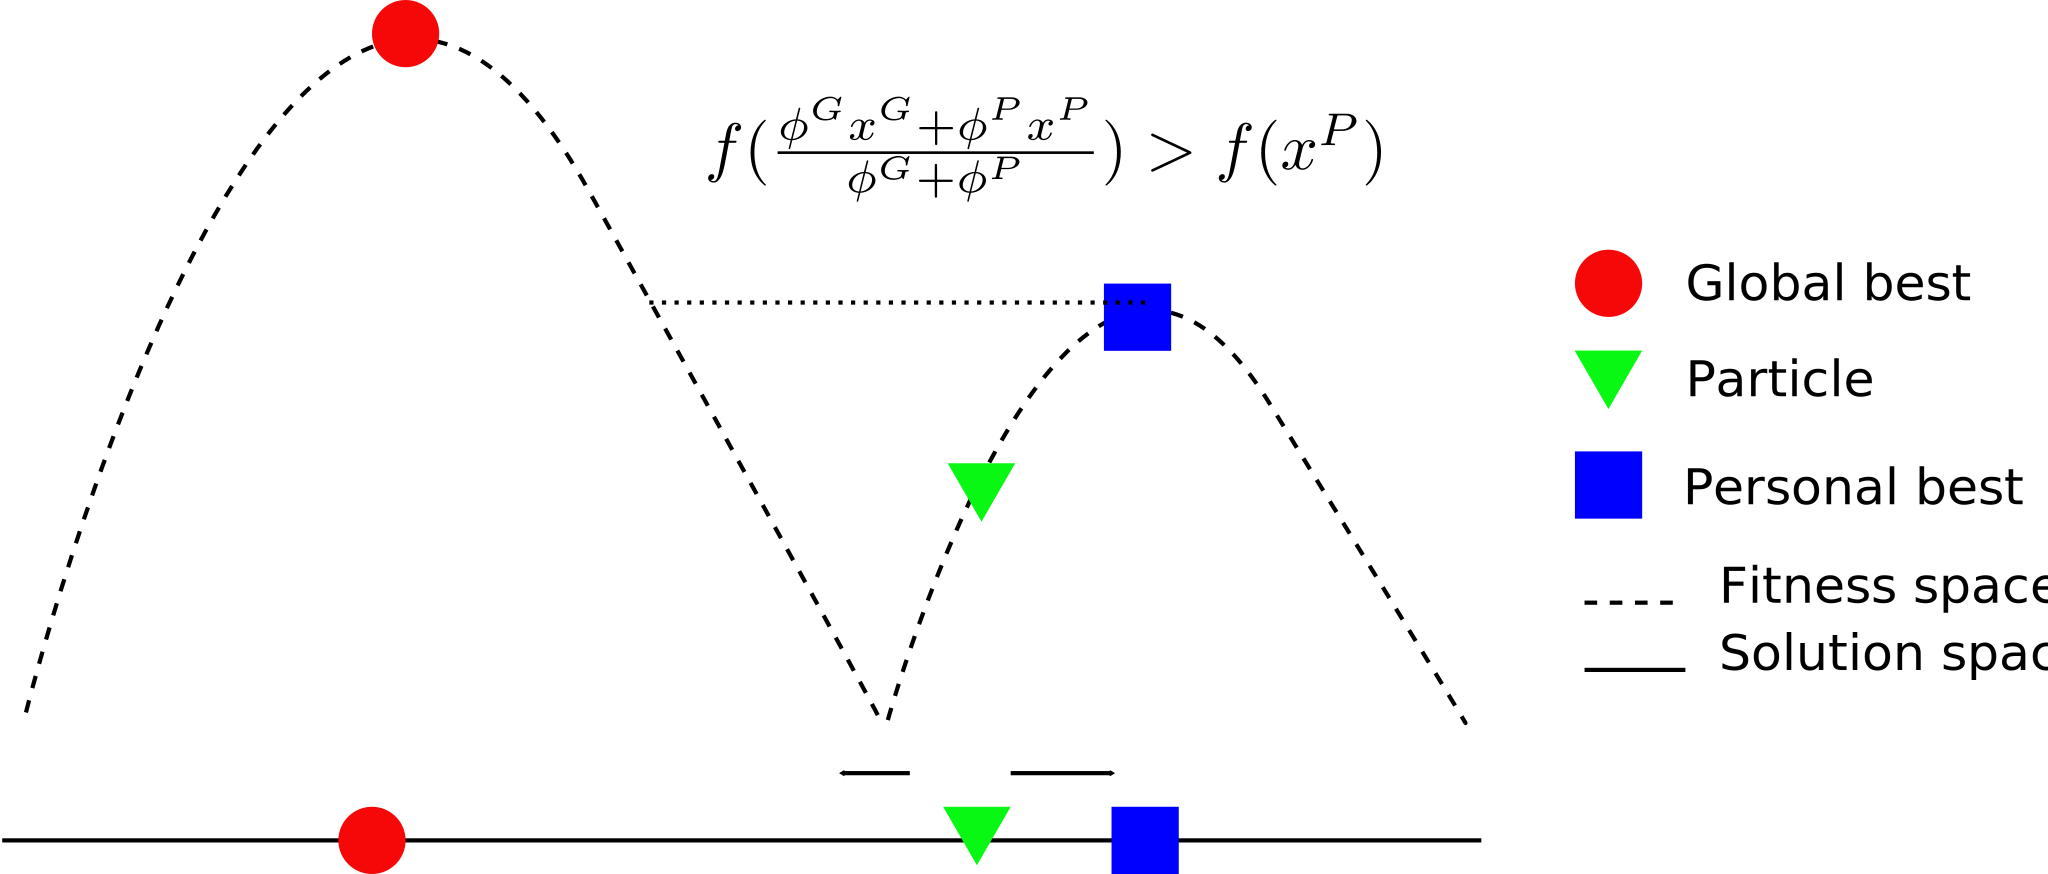
\includegraphics[width=0.57\textwidth]{two_hills_case}
}
\subfigure[The likelihood of moving to the personal best.] {\label{fig:two_hills_case:b}
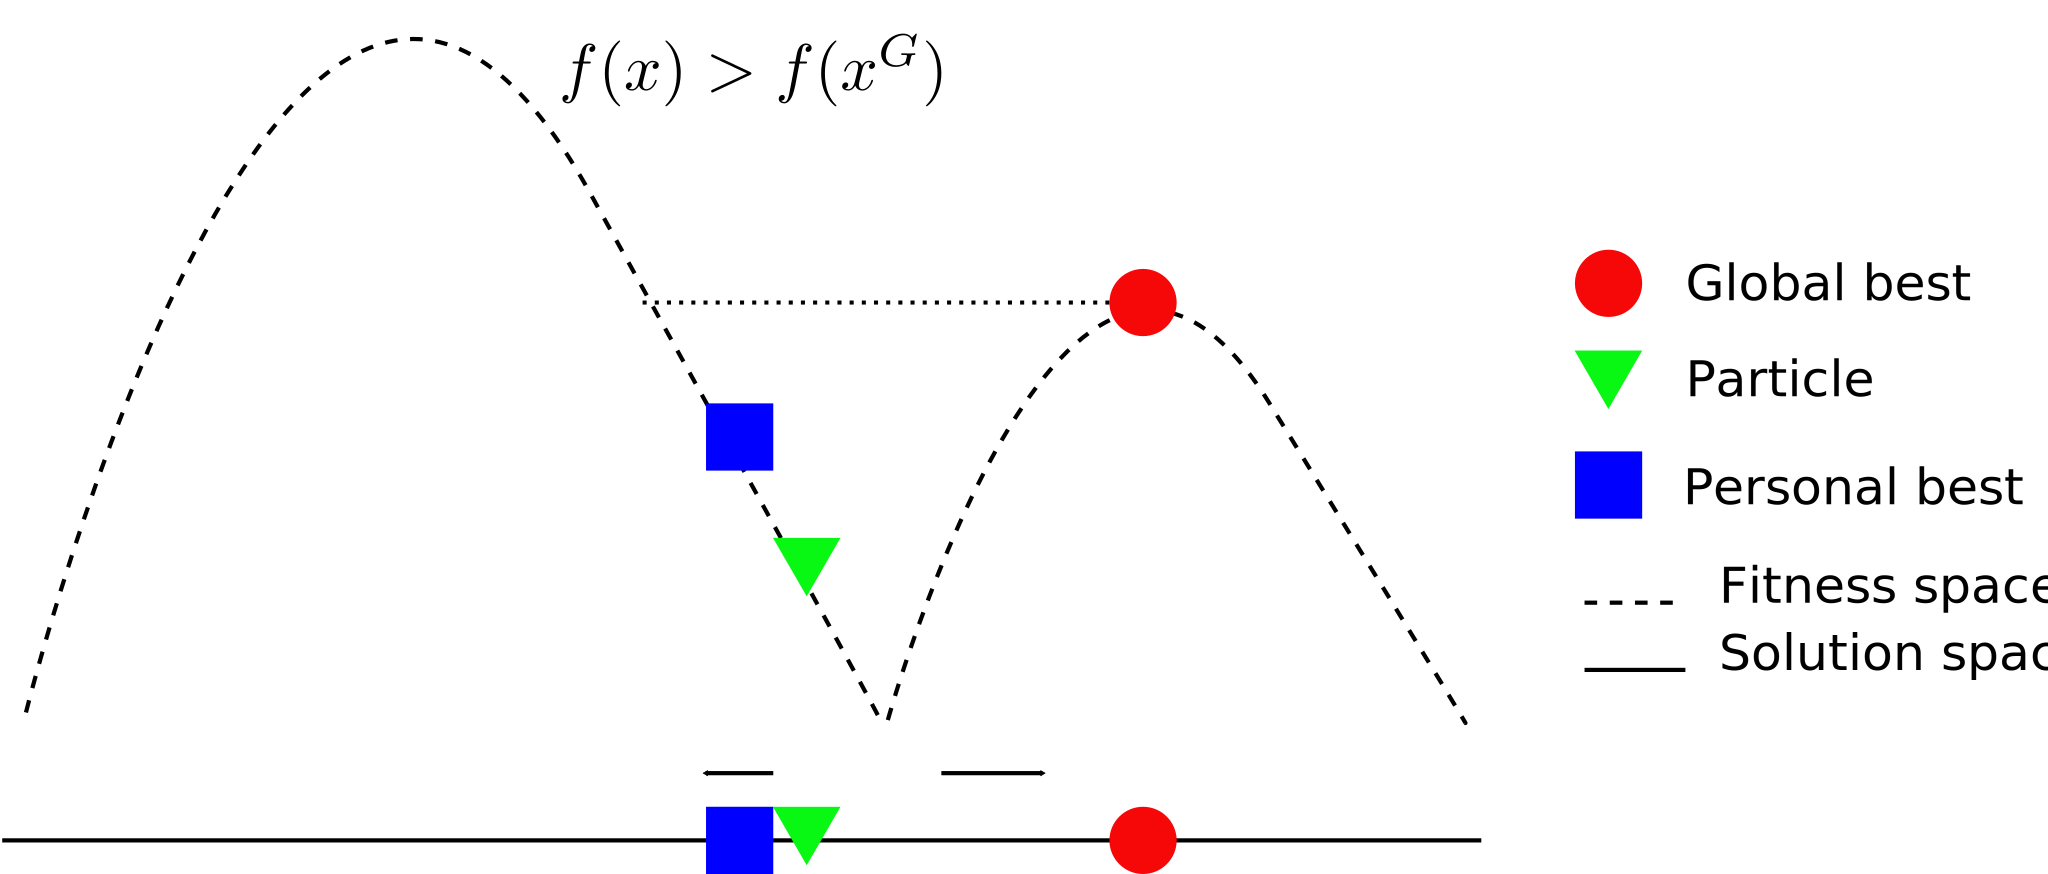
\includegraphics[width=0.57\textwidth]{two_hills_case2}
}
\caption{Two hill case.}
\label{fig:two_hills_case}
\end{figure}


\begin{theorem}
There is a probability $ p $  that a particle moves toward the personal best, and $ 1 - p $ that a particle moves toward the global best,
\begin{equation}
p = 
\end{equation}
\end{theorem}

\begin{corollary}
There is probability $ p $ that the personal best can move to the same hill with the global best,
\begin{equation}
p = 
\end{equation}
\end{corollary}